\documentclass[12pt, a4paper]{article}
\usepackage[utf8]{inputenc}
\usepackage[brazilian]{babel}
\usepackage{geometry}
\usepackage{graphicx}
\usepackage{listings}
\usepackage{xcolor}
\usepackage{hyperref}

\geometry{top=3cm, bottom=2.5cm, left=3cm, right=3cm}

\definecolor{codegreen}{rgb}{0,0.6,0}
\definecolor{codegray}{rgb}{0.5,0.5,0.5}
\definecolor{codepurple}{rgb}{0.58,0,0.82}
\definecolor{backcolour}{rgb}{0.95,0.95,0.92}

\lstdefinestyle{mystyle}{
	backgroundcolor=\color{backcolour},   
	commentstyle=\color{codegreen},
	keywordstyle=\color{magenta},
	numberstyle=\tiny\color{codegray},
	stringstyle=\color{codepurple},
	basicstyle=\ttfamily\footnotesize,
	breakatwhitespace=false,         
	breaklines=true,                 
	captionpos=b,                    
	keepspaces=true,                 
	numbers=left,                    
	numbersep=5pt,                   
	showspaces=false,                
	showstringspaces=false,
	showtabs=false,                  
	tabsize=2
}

\lstset{style=mystyle}

\title{Relatório Técnico: Prototipagem do Sistema de Investimentos VcRiquinho}
\author{Hálan William da Costa Sousa}
\date{}

\begin{document}
	
	\maketitle
	
	\begin{abstract}
		Este documento apresenta a especificação técnica e o relatório de design para o protótipo do sistema de gestão e alocação de investimentos da startup "VcRiquinho". O projeto foi desenvolvido utilizando os princípios de Programação Orientada a Objetos (POO) em Java, integrando uma arquitetura separada em \textit{model}, \textit{view} e \textit{controller}, em camadas com persistência em banco de dados MySQL via \textit{Stored Procedures}, cobrindo o gerenciamento de clientes (Pessoa Física e Jurídica), contas bancárias com regras de rendimento específicas, e produtos financeiros de renda fixa e variável.
	\end{abstract}
	
	\section{Introdução e Contextualização}
	A startup de investimentos \textit{VcRiquinho} iniciou suas operações com o modelo de negócio voltado à gestão e alocação estratégica de recursos de clientes conforme perfis específicos de investimento. O lucro da empresa obtém-se através de taxas de serviço aplicadas sobre os rendimentos obtidos ao longo de períodos arbitrários. Para validar essa proposta, desenvolveu-se um protótipo integrado de linha de comando conectado a um banco de dados relacional, abrangendo o gerenciamento completo (CRUD) de clientes, contas e produtos financeiros, além da simulação de rendimentos e taxas de serviço. Além disso, como requisitado, implementou-se um CRUD para gerenciamento dos produtos de investimento.
	
	\section{Decisões de Design (Arquitetura Orientada a Objetos e Banco de Dados)}
	Para assegurar a manutenibilidade, a robustez e a aderência aos requisitos do projeto, adotou-se uma arquitetura estruturada em pacotes (\texttt{model},\texttt{view}, \texttt{controller} e \texttt{dao}).
	
	\begin{itemize}
		\item \textbf{Hierarquia de Clientes e Contas:} Utilização de classes abstratas e herança para separar \texttt{IndividualClient} (PF) e \texttt{CorporateClient} (PJ) sob a superclasse \texttt{Client}, bem como diferentes modalidades de contas (\texttt{CheckingAccount}, \texttt{CdiAccount} e \texttt{AutoInvestmentAccount}) estendendo \texttt{BaseAccount} que implementa a interface \texttt{Account}.
		\item \textbf{Polimorfismo para Rendimentos e Taxas:} Aplicação de métodos polimórficos de cálculo de rendimento (\texttt{calculateYield}) e taxas de serviço (\texttt{calculateServiceFee}) com base na tipagem dinâmica das contas e dos produtos financeiros associados.
		\item \textbf{Persistência com Stored Procedures:} O acesso aos dados isola as regras de negócio do banco de dados relacional \texttt{vcRiquinhoDB} por meio de procedimentos armazenados (\textit{Stored Procedures}), garantindo transacionabilidade segura e integridade referencial com restrições \texttt{ON DELETE CASCADE}, que garante que os relacionamentos que surgem para adequar o modelo orientado à objetos ao relacional sejam apagados em caso do apagamento do registro no banco.
	\end{itemize}
	
	\section{Descrição do Funcionamento do Sistema}
	O fluxo operacional do sistema contempla as seguintes etapas principais:
	\begin{enumerate}
		\item \textbf{Autenticação e Cadastro:} O operador realiza o cadastro de clientes (PF ou PJ) via \texttt{ClientController} e procedimento armazenado \texttt{CADASTRO\_CLIENTE}, ou efetua o \textit{login} populando dinamicamente o objeto \texttt{Client} e suas respectivas contas associadas.
		\item \textbf{Gestão de Contas e Produtos:} O sistema permite a criação de novas contas vinculadas ao cliente e o gerenciamento de produtos de investimento de Renda Fixa (com período de carência) e Renda Variável.
		\item \textbf{Simulação de Rendimentos:} Através de parâmetros de tempo (30, 60, 90 ou 120 dias), o sistema calcula rendimentos e aplica as taxas específicas (ex.: 0,07\% para CDI; 0,1\% para PF e 0,15\% para PJ em contas de auto-investimento), desconsiderando automaticamente produtos de renda fixa que se encontrem dentro do período de carência.
	\end{enumerate}
	
	\section{Exemplo de Código do Protótipo}
	Abaixo encontra-se parte da implementação do controlador \texttt{ClientController}, responsável pelo gerenciamento e simulação das regras de negócio das contas:
	
	\begin{lstlisting}[language=Java, caption=Trecho do ClientController.java]
		public void calcularRendimento(Client cli, String id, int dias) {
			for (BaseAccount acc : cli.getAccounts()) {
				if (acc.getId().equalsIgnoreCase(id)) {
					if (acc instanceof CheckingAccount) {
						System.out.println("Rendimento: " + 
						((CheckingAccount) acc).calculateYield(dias));
					} else if (acc instanceof CdiAccount) {
						System.out.println("Rendimento: " + 
						((CdiAccount) acc).calculateYield(dias));
					} else if (acc instanceof AutoInvestmentAccount) {
						System.out.println("Rendimento: " + 
						((AutoInvestmentAccount) acc).calculateYield(dias));
					}
					return;
				}
			}
			System.out.println("Conta nao encontrada");
		}
	\end{lstlisting}
	
	\section{Modelagem do Banco de Dados e Diagramas}
	O sistema é sustentado por um esquema relacional normalizado no MySQL (\texttt{vcRiquinhoDB}), compreendendo tabelas estruturadas para clientes, especializações PF/PJ, contas bancárias, contas auxiliares (CDI e Auto-Investimento) e produtos financeiros com suas respectivas restrições de renda fixa e variável.
	Para compreender melhor a modelagem da parte orientada à objetos desse sistema foi desenvolvido um diagrama de classes UML.
	
	\begin{figure}[htbp]
		\centering
		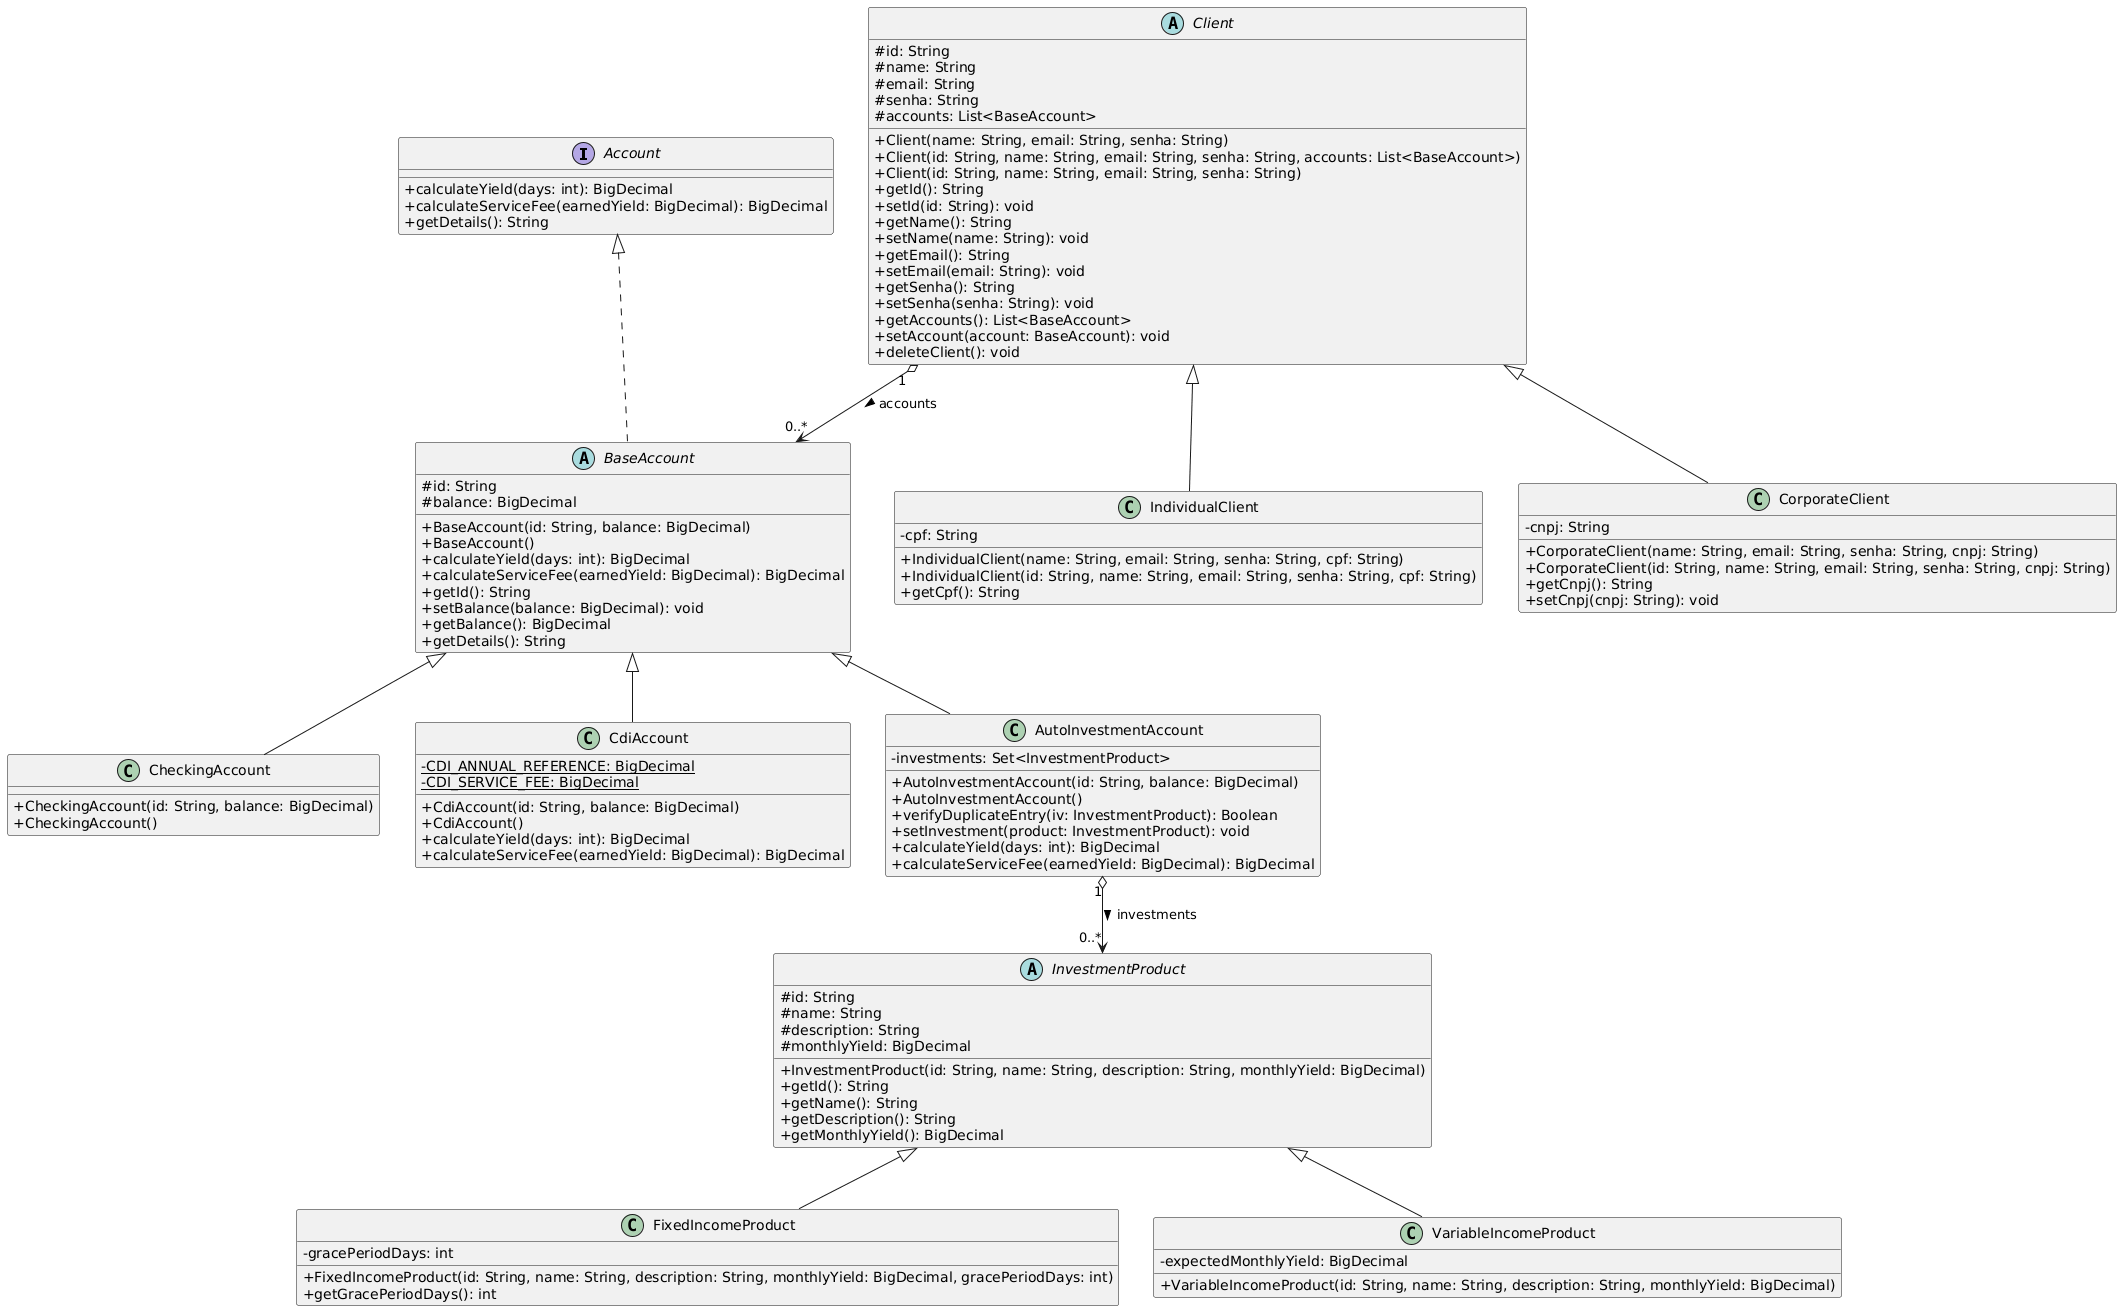
\includegraphics[width=1\textwidth]{img/diagrama_classes.png}
		\caption{Diagrama UML}
		\label{fig: Diagrama de classes UML}
		
	\end{figure}
	
	\section{Considerações Finais}
	O protótipo desenvolvido cumpre integralmente os requisitos funcionais e técnicos estipulados para a startup \textit{VcRiquinho}. A sinergia entre os conceitos avançados de Orientação a Objetos em Java e a persistência orientada a procedimentos armazenados em banco de dados assegura uma base sólida, extensível e segura para futuras expansões comerciais e operacionais da plataforma.
	
\end{document}